\documentclass[a4paper, 11pt]{article}
\usepackage[utf8]{inputenc}
\usepackage[T1]{fontenc}
\usepackage[francais]{babel}
\usepackage[top=3cm, bottom=4cm, left=3cm, right=3cm]{geometry}
\usepackage{graphicx}
\usepackage[babel=true]{csquotes}
\usepackage{titlesec}
\usepackage{url}
\usepackage{hyperref}

\setcounter{secnumdepth}{3} % On affiche une numérotation sur une profondeur de 3
\setcounter{tocdepth}{3} % La table des matières va a une profondeur de 3
\titlespacing{\chapter} {0pt} {*0} {*0} {}



\title{\textbf{Rapport}\\\Large{Extraction de connaissances avancée}}
\author{Jessie CARBONNEL, Daniel NGUYEN \& Lionel PIBRE}
\date{\textit{Jeudi 11 décembre 2014} \\ 
\includegraphics[height=.13\textheight]{um2.jpg}\\[1cm]}

\begin{document}
\maketitle

\section{Présentation}
Ce projet s'inscrit dans le cadre de l'UE GMIN313 Extraction de connaissances avancée et a pour but d'appliquer les différentes techniques de fouille et d'analyse de données vues en cours.\\

\textbf{Contraintes} : L'analyse doit s'effectuer sur des données textuelles hétérogènes et doit porter sur des sentiments ou des opinions.

\section{Outils utilisés}
Voici la liste des différents outils utilisés lors de ce projet : 
\begin{itemize}
\item \textbf{Hadoop MapReduce} pour une partie analyse de données nettoyées avant la visualisation,
\item \textbf{D3.js} pour produire une visualisation web grâce aux données analysées,
\item \textbf{TreeTagger} pour préparer le corpus en étiquetant le texte donné,
\item \textbf{API Weka} pour appliquer les algorithmes de fouilles de données,
\item \textbf{Langage de programmation : Java} pour manipuler les fichiers
\end{itemize}

\section{Constitution du corpus}

Nous avons décidé de travailler sur un corpus basé sur des commentaires d'applications Android.

Nous avons choisi de les extraire depuis les applications disponibles sur le Google Play Store (\url{https://play.google.com/store/apps}) : les applications y sont nombreuses, variées et le site possède une communauté importante.
Les informations relatives à un commentaire sont les suivantes : le contenu de la description, le titre, la note de l'application et la date. Nous pouvons aussi utiliser des informations relatives à l'application pour les mettre en parallèle avec les commentaires : la note globale, le nombre de votants, la catégorie ...
On peut trouver diverses API qui permettent de récupérer les informations relatives aux applications de Google Store. Nous avons choisi une API non officielle, \textit{Android Market API}, qui est rapide à prendre en main et permet d'extraire facilement les commentaires.

Chaque API possède un identifiant unique. Nous avons donc dans un premier temps récupérer les identifiants de 135 applications dans des sections variées. Puis nous avons récupéré les informations des 40 derniers commentaires de chacune de ces applications.

Chaque commentaire va faire l'objet d'un fichier. Voici l'exemple, récupéré via l'API, des informations relatives au premier commentaire d'une application permettant de lire des PDF (\textit{books.ebook.pdf.reader\#1.txt}) :

\begin{verbatim}
NomApplication:Ebook et PDF Reader
IdApplication:books.ebook.pdf.reader
CategorieApplication:Livres et références
NoteApplication:4,3
NombreVotants:43 379
TitreCommentaire:Ebook Pelerin
Commentaire: Super installation, ai acheté un ebook chez Bayard. Suis pas déçu.
DateCommentaire:26 juillet 2014
NoteCommentaire:5
\end{verbatim}


Nous avons extrait un total de 5346 commentaires dans ce format.

\section{Préparation des données}

\subsection{TreeTagger}
Afin de réaliser le prétraitement sur notre corpus, nous avons utilisé TreeTagger. Ce logiciel nous permet de connaître la classe grammaticale des mots et d’obtenir la forme lemmatisée de ces derniers. Cet outil nous a permis de nettoyer le corpus en supprimant par exemple les pronoms et les déterminants.

La figure \ref{treetagger} présente un exemple de TreeTagger.
\newpage
\begin{figure}[!h]
\centering
 \begin{tabular}{|c|c|c|}
 \hline
	Mot&Classe grammaticale&Mot lemmatisé\\
 \hline
    dès&PRP&dès\\
    que&KON&que\\
    je&PRO:PER&je\\
    lance&VER:pres&lancer\\
    l'&DET:ART&le\\
    application&NOM&application\\
    ça&PRO:DEM&cela\\
    marche&NOM&marche\\
    pas&ADV&pas\\
    sinon&KON&sinon\\
    j'&PRO:PER&je\\
    adore&VER:pres&adorer\\
    cyprien&ADJ&cyprien\\
    \dots&\dots&\dots\\
 \hline
 \end{tabular}
 \caption{Exemple de TreeTagger}
\label{treetagger}
\end{figure}

\subsection{Génération des fichiers ARFF avec un parser Java}
 
Nous utilisons l'API java.nio, développée pour JDK7, qui facilite la manipulation d'entrées/sorties de système de fichiers et qui accorde une importance à la scalabilité.
 
En entrée les données étiquetées par TreeTagger, en sortie un fichier de format ARFF. Un fichier ARFF est un simple fichier texte structuré de façon à être lisible par le programme Weka.

On récupère la ligne \textit{NoteCommentaire}, et le texte entre \textit{TitreCommentaire} et \textit{DateCommentaire}. La valeur associée à \textit{NoteCommentaire} est entre 1 et 5, représentée sous forme de nombre d'étoiles dans le Play Store, et va nous permettre de catégoriser le commentaire dans une des trois classes d'opinion :
\begin{itemize}
        \item{[1,2]} = mauvais
   \item{3} = neutre
   \item{[4,5]} = bien
\end{itemize}
Une fois le commentaire catégorisé dans une des classes, les mots contenus dans ce commentaire seront utilisés afin de créer une caractéristique ou bien une règle à la classe pour, ensuite, bien classer un nouveau commentaire entrant. Cette étape sera détaillée par la suite dans la section \ref{fouille}.
 
 
Pour le commentaire etiqueté dans la figure \ref{treetagger}, avec une valeur de \textit{NoteCommentaire} à 3, nous aurons la ligne suivante :
\begin{verbatim}
neutre, 'bug lancement lancer application marche help adorer cyprien ...'
\end{verbatim}
 
Notre fichier ARFF contiendra 5346 lignes dans ce format et sera utilisé pour effectuer une première analyse visualisable, mais aussi pour mettre en pratique les algorithmes de fouilles de données.

Nous avons décidé de créer huit fichiers ARFF différents afin de voir l'impact qu'a la composition du corpus sur les algorithmes de classification.

\begin{itemize}
 \item Le texte brut (sans aucune modification)
 \item Le texte brut en utilisant la forme lemmatisée des mots
 \item Le texte uniquement composé d'adjectifs, de noms et de verbes
 \item Le texte uniquement composé d'adjectifs, de noms et de verbes en utilisant la forme lemmatisée des mots
 \vspace{0.5cm}
 \item Ensuite, nous avons repris ces quatre fichiers ARFF mais en corrigeant l'orthographe des verbes aimer et adorer, nous avons aussi remplacer ``kiffer'' par aimer.
\end{itemize}

\section{Analyse et visualisation des données}
 

 
\subsection{Statistiques sur les données préparées}\label{sec:visu-process}
 
Nous allons exécuter deux processus
\paragraph{Compter la part de chaque classe} avec une méthode qui compte le nombre total de commentaire classé "bien", "neutre" et "mauvais" : on calcule le pourcentage que représente chaque classe on peut observer une majorité absolue pour la classe "bien" (3279 commentaires positifs pour 5346, soit 61\%).
 
\paragraph{Lister les mots les plus fréquents de chaque classe} en utilisant le framework Hadoop MapReduce que nous avons au préalable mis en place dans une autre UE pour exécuter cette même tâche : nous avons un programme qui va se charger de lire, dans le fichier ARFF précédent, les lignes qui commencent par "bien", "neutre" et "mauvais" puis de compter l'occurrence de chaque mot et les trier par ordre décroissant dans chacune des classes.
 
\subsection{Résultats obtenus avec Hadoop}
Nous avons réussi à extraire la liste des 5 mots les plus utilisés par classe dans les commentaires.

Ils sont présentés dans la figure \ref{mots les plus utilisés}.

\begin{figure}[h]
\begin{center}


\begin{tabular}{|l|c|c|}
\hline
Classe &	Mot&	Valeur\\
\hline
\hline
bien&	cool&	578\\
\hline
bien&	super&	481\\
\hline
bien&	bon	&455\\
\hline
bien&	adorer&	25\\
\hline
bien&	merci&	219\\
\hline
\hline
neutre&	jour&	96\\
\hline
neutre&	bon	&72\\
\hline
neutre&	mise&	61\\
\hline
neutre&	mettre&	58\\
\hline
neutre&	dommage	&54\\
\hline
\hline
mauvais&	jour&	-271\\
\hline
mauvais	&nul	&-242\\
\hline
mauvais	&impossible	&-189\\
\hline
mauvais	&fonctionner&	-182\\
\hline
mauvais	&mettre&	-174\\
\hline
\end{tabular}
\end{center}
\caption{Top 5 des mots les plus utilisés dans chaque classe}
\label{mots les plus utilisés}
\end{figure}
 
\subsection{Visualisation avec D3.js}
 
Nous allons visualiser les statistiques de la section \ref{sec:visu-process} en utilisant la librairie D3.js pour produire des figures à partir des données récupérées.
 
\paragraph{Une première visualisation en camembert}pour représenter le pourcentage des commentaires appartenant à chaque classe : \textit{bien}, \textit{mauvais} ou \textit{neutre}. Ces résultats sont représentés dans la figure \ref{camembert}.\\
\paragraph{Une seconde en histogramme}pour mettre en évidence les mots les plus présents dans chaque classe, et donc voir les mots les plus caractéristiques d'une opinion dans notre corpus. Ces résultats sont représentés dans la figure \ref{histogramme}.

\begin{figure}[h]
\begin{center}
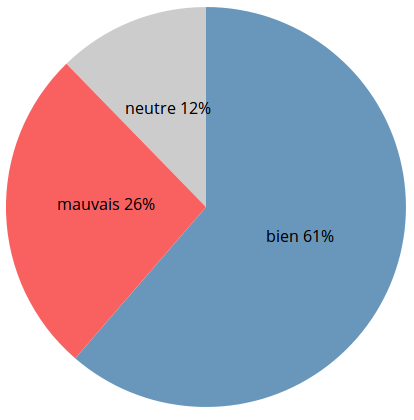
\includegraphics[width=0.4\textwidth]{visu1.png}
\end{center}
\caption{Pourcentage des commentaires en fonction de leur classe}\label{camembert}
\end{figure}

\begin{figure}[h]
\begin{center}
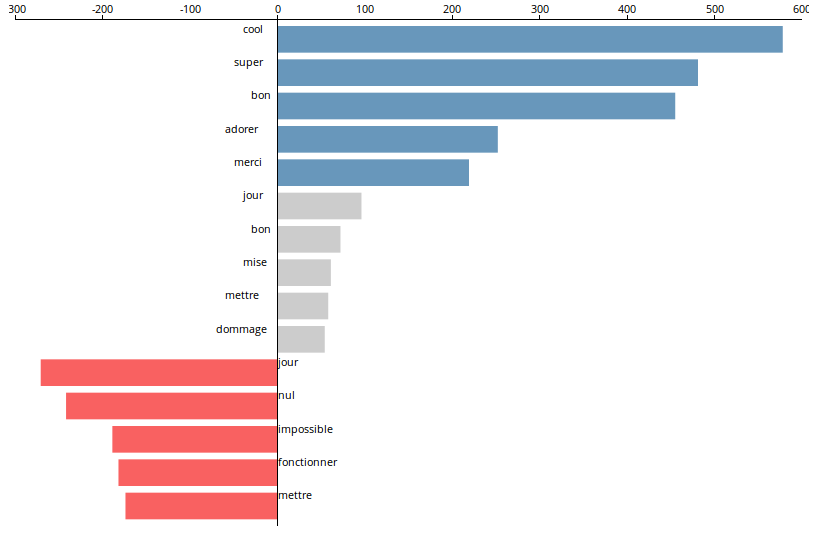
\includegraphics[width=\textwidth]{visu2.png}
\end{center}
\caption{Top 5 des mots les plus utilisés dans chaque classe et leur nombre d'occurence}\label{histogramme}
\end{figure}
\clearpage

\section{Fouille de données}\label{fouille}

Voici les différents algorithmes appliqués avec Weka dans la partie fouille de données : \\

\begin{description}
 \item [NaiveBayes: ] la classification naïve bayésienne est un type de classification probabiliste simple basée sur le théorème de Bayes avec une forte indépendance des hypothèses. \\

 \item [Arbre de décision (J48): ] cet algorithme utilise une structure d'arbre. L'extrémité de chaque branche représente les différents résultats possibles en fonction des décisions prises à chaque étape. Cet algorithme  répartit une population d'individus en groupes homogènes, selon un ensemble de variables discriminantes en fonction d'un objectif fixé et connu.\\

 \item [SVM (SMO): ] Les SVM sont des classificateurs qui reposent sur deux idées-clés:

\begin{itemize}
 \item La notion de marge maximale. La marge est la distance entre la frontière de séparation et les échantillons les plus proches.
Ces derniers sont appelés vecteurs supports. Dans les SVM, la frontière de séparation est choisie comme celle qui maximise la marge.
Le problème est de trouver la frontière séparatrice optimale, à partir d'un ensemble d'apprentissage. Cependant il existe déjà des algorithmes pour résoudre ce problème
 \item  Transformer l'espace de représentation des données d'entrées en un espace de plus grande dimension, dans lequel il est probable qu'il existe une séparatrice linéaire. \\
\end{itemize}
 \item [Méthode par règles d'association (JRip): ] La méthode par règles d’association s’apparente à celle des arbres de décision. Chaque règle pouvant être vue comme le parcours dans un arbre de décision binaire. Cependant les arbres de décisions essayent de réduire le nombre de parcours à explorer tandis qu’ici on explore tout.\\

 \item [K plus proche voisin (IBk): ] L’algorithme KNN figure parmi les plus simples algorithmes d’apprentissage artificiel. Dans un contexte de classification d’une nouvelle observation x, l’idée fondatrice simple est de faire voter les plus proches voisins de cette observation. La classe de $x$ est déterminée en fonction de la classe majoritaire parmi les k plus proches voisins de l’observation $x$. La méthode KNN est donc une méthode à base de voisinage, non-paramétrique ; Ceci signifiant que l’algorithme permet de faire une classification sans faire d’hypothèse sur la fonction $y=f(x_1,x_2,…x_p)$ qui relie la variable dépendante aux variables indépendantes.
\end{description}

\section{Résultats}

\subsection{Résultats obtenus avec Weka}

Les tableaux suivant représentent les résultats des instances correctement classifiées (en pourcentage). Pour obtenir ces résultats nous avons utilisé une représentation de type ``sac de mots''. Nous avons donc utilisé le filtre de Weka ``StringToWordVector'', d'abord sans l'option ``outputWordCounts'' (les résultats de la colonne binaire), puis en activant cette option (la colonne fréquence).

\subsubsection{Texte non corrigé}
\begin{figure}[h]
\begin{minipage}{0.5\textwidth}
\begin{tabular}{|c|c|c|}
\hline
 & Binaire & Fréquence \\
 \hline
 NaiveBayes & 64.1788 & 63.6551 \\
 \hline
 SMO & 73.1201 & 73.6438 \\
 \hline
 IBk & 65.563 & 64.3659 \\
 \hline
 J48 & 67.8451 & 67.8638 \\
 \hline
 JRip & 64.7961 & 65.2637 \\
 \hline
\end{tabular}
\caption{Texte brut}
\end{minipage}
\begin{minipage}{0.5\textwidth}
\begin{tabular}{|c|c|c|}
\hline
 & Binaire & Fréquence \\
 \hline
 NaiveBayes & 65.8997 & 65.376 \\
 \hline
 SMO & 73.6438 & 74.3172 \\
 \hline
 IBk & 65.9371 & 64.4407 \\
 \hline
 J48 & 68.9113 & 68.7991 \\
 \hline
 JRip & 67.7703 & 68.3315 \\
 \hline
\end{tabular}
\caption{Texte brut lemmatisé}
\end{minipage}
\end{figure}
\vspace{1cm}
\begin{figure}[h]
\begin{minipage}{0.5\textwidth}
\begin{tabular}{|c|c|c|}
\hline
 & Binaire & Fréquence \\
 \hline
 NaiveBayes & 66.517 & 65.4321 \\
 \hline
 SMO & 72.5776 & 72.5963 \\
 \hline
 IBk & 64.5342 & 64.1227 \\
 \hline
 J48 & 69.2854 & 69.0797 \\
 \hline
 JRip & 66.33 & 65.9559 \\
 \hline
\end{tabular}
\caption{Texte nettoyé}
\end{minipage}
\begin{minipage}{0.5\textwidth}
\begin{tabular}{|c|c|c|}
\hline
 & Binaire & Fréquence \\
 \hline
 NaiveBayes & 67.9012 & 66.4796 \\
 \hline
 SMO & 72.8021 & 73.2697 \\
 \hline
 IBk & 65.9746 & 62.1212 \\
 \hline
 J48 & 69.0423 & 68.9862 \\
 \hline
 JRip & 67.5832 & 67.5645 \\
 \hline
\end{tabular}
\caption{Texte nettoyé lemmatisé}
\end{minipage}
\end{figure}
\subsubsection{Texte corrigé}
\begin{figure}[h]
\begin{minipage}{0.5\textwidth}
\begin{tabular}{|c|c|c|}
\hline
 & Binaire & Fréquence \\
 \hline
 NaiveBayes & 64.2724  & 63.6177 \\
 \hline
 SMO & 73.1949 & 73.569 \\
 \hline
 IBk & 65.6004 & 64.3659 \\
 \hline
 J48 & 67.8077 & 67.8451 \\
 \hline
 JRip & 65.2263 & 65.7127 \\
 \hline
\end{tabular}
\caption{Texte brut}
\end{minipage}
\begin{minipage}{0.5\textwidth}
\begin{tabular}{|c|c|c|}
\hline
 & Binaire & Fréquence \\
 \hline
 NaiveBayes & 66.0307 & 65.5256 \\
 \hline
 SMO & 73.4755 & 74.6914 \\
 \hline
 IBk & 66.0307 & 64.3285 \\
 \hline
 J48 & 69.5099 & 69.2667 \\
 \hline
 JRip & 67.4336 & 67.3588 \\
 \hline
\end{tabular}
\caption{Texte brut lemmatisé}
\end{minipage}
\end{figure}
\newpage
\begin{figure}[h]
\begin{minipage}{0.5\textwidth}
\begin{tabular}{|c|c|c|}
\hline
 & Binaire & Fréquence \\
 \hline
 NaiveBayes & 66.835 & 65.4134 \\
 \hline
 SMO & 72.1848 & 72.4654 \\
 \hline
 IBk & 64.7774 & 64.7026 \\
 \hline
 J48 & 69.3229 & 69.3042 \\
 \hline
 JRip & 66.3113 & 65.9746 \\
 \hline
\end{tabular}
\caption{Texte nettoyé}
\end{minipage}
\begin{minipage}{0.5\textwidth}
\begin{tabular}{|c|c|c|}
\hline
 & Binaire & Fréquence \\
 \hline
 NaiveBayes & 67.8077 & 66.7228 \\
 \hline
 SMO & 73.6064 & 73.251 \\
 \hline
 IBk & 64.4407 & 63.3184 \\
 \hline
 J48 & 69.2854 & 69.5099 \\
 \hline
 JRip & 67.7142 & 67.3588 \\
 \hline
\end{tabular}
\caption{Texte nettoyé lemmatisé}
\end{minipage}
\end{figure}


\section{Analyse des résultats}

\subsection{Analyse des résultats de Weka}
Comment expliquer que les résultats obtenus soient aussi bas?\\

Lorsque nous avons fait le prétraitement, nous avons vu que deux éléments risquaient de limiter nos résultats.

\begin{description}
	\item [Les fautes d'orthographe et de frappe: ]``Je kiff grave car jadore cyprien et jaimefai lui poser un question : est ce que tu connais squeezie ( ca c oui c sur ) norman kihouu tal blackm ....''\\
	
	Dans ce cas, peu de mots sont reconnus par TreeTagger. Par exemple les mots ``kiff'' et ``jadore'' ne sont pas reconnus alors qu'ils déterminent l'opinion de l'utilisateur.
	
	\item [Les commentaires en anglais: ]Certains commentaires sont écrits en anglais et ne sont donc pas reconnus par TreeTagger.
\end{description}

On peut voir d'après les résultats obtenus que l'algorithme de classification le plus efficace est SMO. Cet algorithme est très robuste au bruit et, comme on a pu le constater au vu des résultats, aux fautes d'orthographe.\\

Les algorithmes JRip et J48 ne sont pas efficaces car ils se basent sur des règles afin de déterminer la classe d'un commentaire. En effet, les fautes d'orthographe empêchent de faire des règles précises et efficaces, car un même mot peut être écrit de plusieures manières différentes dans ces commentaires.
On peut aussi voir que le fait que les mots soient représentés par la présence ou l'occurence importe peu, car les résultats diffèrent très peu. \'{E}tant donné que notre corpus contient un nombre incalculable de fautes d'orthographe, la représentation des données n'impacte pas les résultats.\\

NaiveBayes est un algorithme de classification probabiliste, encore une fois les fautes d'orthographe jouent un rôle important dans les résultats de cet algorithme. En effet, les fautes l'empêchent de créer des caractéristiques spécifiques aux différentes classes, puisque les mêmes mots sont écrits de différentes façon dans le corpus.\\

Pour l'algorithme IBk, le fait que des mots apparaissent dans des classes différentes (par exemple le mot ``dommage'', qui apparaît dans toutes les classes), empêche d'obtenir de meilleurs résultats. De plus on peut remarquer que cet algorithme est plus efficace lorsque la représentation des mots est binaire, cela vient du fait que les mots vides ont moins d'importance dans ce cas là.

\subsection{Analyse des mots les plus fréquents}
L'extraction du top 5 des mots les plus utilisés dans chaque classe semble cohérente.

Le mot "\textit{bon}" se retrouve dans la classe bien et neutre, mais pas dans la classe mauvais.

Les personnes satisfaites ont tendance à exprimer leur satisfaction avec des adjectifs ou des verbes positifs (\textit{"cool", "super", "bon", "adorer"}) ainsi que leur gratitude ("\textit{merci}").  

Celles qui ne sont pas satisfaites n'expriment pas seulement leur désapprobation avec des adjectifs négatifs ("\textit{nul}"). Ils ont aussi tendance à expliquer ce qui ne leur convient pas et les problèmes rencontrés avec le fonctionnement de l'application ("\textit{fonctionner}" et "\textit{impossible}"). Les mots "\textit{mettre}" et "\textit{jour}" apparaissent tous deux dans les classes neutre et mauvais. On peut faire l'hypothèse que les individus qui ne laissent pas de bons commentaires tendent à proposer ou demander des "mises à jours" pour l'application. Ce qui n'est pas le cas des personnes qui en sont satisfaites.\\

D'après ces résultats, il semble que si les développeurs d'une application ont besoins de retours utiles sur le fonctionnement de l'application, ils devraient regarder les commentaires les plus négatifs en premier.

\section{Conclusion et perspectives}
\subsection{Conclusion}
Nous avons travaillé sur un corpus de plus de 5000 commentaires portant sur un ensemble d'applications variées. 

Nous avons extrait pour chaque classe de commentaire (bon, neutre ou mauvais) les cinq mots les plus fréquemments utilisés. Nous avons émis des hypothèses sur l'importance de la dimension critique des commentaires rédigés par des utilisateurs qui ont une mauvaise opinion de l'application par rapport à ceux rédigés par des utilisateurs satisfaits.

Nous avons utilisé des techniques de visualisation pour montrer la proportion des trois classes de commentaires ainsi que la fréquence des mots les plus utilisés.

Puis nous avons appliqué les algorithmes de classification sur les fichiers ARFF obtenus après le prétraitement des données que nous avons effectué sur le corpus.

Enfin, nous avons analysé les résultats obtenus.

\subsection{Perspectives}
Utiliser des outils de TALN afin de corriger le corpus ainsi que traduire les commentaires en anglais. En effet, on peut remarquer dans les résultats que juste le fait de corriger l'orthographe de trois verbes, les algorithmes obtiennent pour la majorité d'entre eux de meilleurs résultats.

Visualiser les résultats obtenus après la fouille de données pour comparer les algorithmes.

Tester d'autres algorithmes afin de voir s'il n'y a pas un ou plusieurs algorithmes plus performants que ceux testés au cours de ce projet.

\end{document}

